\ocumentclass[a4paper,10pt]{article}

\usepackage[utf8]{inputenc}
\usepackage{natbib}
\usepackage[vmargin=2cm]{geometry}
\usepackage{csvsimple}

\setlength{\bibsep}{1pt}
\usepackage{graphicx}
\graphicspath{{Figures/}}

\usepackage{hyperref}
\hypersetup{
  colorlinks, linkcolor=red
}

\renewcommand{\bibfont}{\small}


%\title{Project report - Object Recognition and Computer vision}
\title{%
	\huge{Assembling LEGO set with augmented reality instructions}\\ \bigbreak
  	\Large{Project report}\\ 
  	\Large{Object Recognition and Computer vision - MVA}
}
\author{Othman Sbai, Pierre-Alain Langlois}
\date\today

\pdfinfo{%
  /Title    (Project report - Computer vision - Sbai & Langlois)
  /Author   (Othman Sbai, Pierre-Alain Langlois)
  /Creator  (Pierre-Alain Langlois, Othman Sbai)
  /Subject  (Augmented reality - tracking)
  /Keywords (augmented reality neural network ponts)
}

\begin{document}

\maketitle

\section{Introduction}
The advent of augmented reality devices such as Microsoft Hololens, Sony SmartEyeglass or Google Glass and others have made possible many interesting applications that augment the visual experience of the user with 3D holograms that are blended on his reality. Applications range from interior decoration and design, gaming but also increasing productivity in businesses by enhancing the real world and giving birth to broader imagination.

Among the applications of this new promising technology still in development, one can be interested providing instructions for people to help them accomplish tasks either with human supervision or by annotating reality. In fact, as presented in \cite{alayrac_unsupervised_2015}, we can extract from the tutorial videos available online instructions for performing many tasks such as changing car tires, assembling furniture and also performing Cardiopulmonary rescucitation. These instructions can be efficiently provided to user with a 3D augmented reality device in the form of holograms and world annotations that are much comprehensible than paper instructions. An example of this world annotation is illustrated in the following figure~\ref{AnnotatingTheWorld}.


\begin{figure}
    \centering
    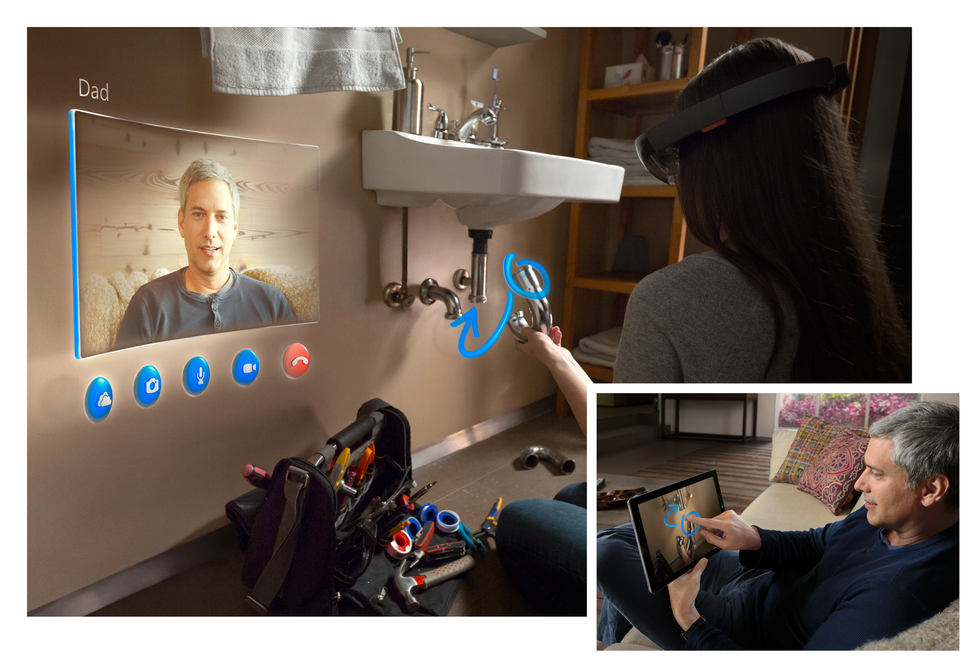
\includegraphics[width=0.75\textwidth]{Annotating_world_hololens}
    \caption{Annotating the world with Microsoft Hololens}
    \label{AnnotatingTheWorld}
\end{figure}

\section{Approach of the project}
As a simplified approach to the problem providing holographic instructions as described before, we set to work on the assembly of a LEGO set using a Microsoft Hololens device to visualize the created 3D holograms and assessing the created experience. 

\subsection{Lego set description} % parts and choice ...
In coordination with other group of students working on a similar project topic, we decided to choose the LEGO set named "Blue racer" (ref 31027) shown in figure~\ref{BlueRacer}
\begin{figure}
    \centering
    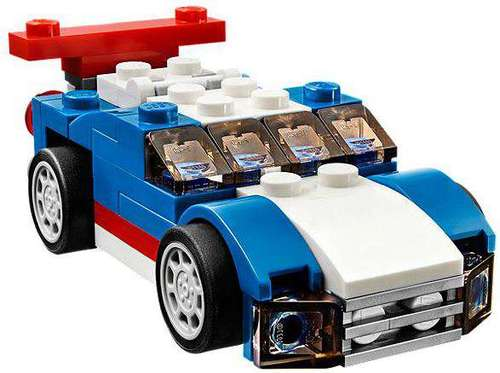
\includegraphics[width=0.5\textwidth]{BlueRacer}
    \caption{Lego set chosen for this project}
    \label{BlueRacer}
\end{figure}

\section{Introduction to Hololens device}

\subsection{Working with hololens}

Microsoft Hololens is not a cheap platform to work on as it cost at least 3000\$. Thankfully, there is the possibility of working on an emulator for hololens on Visual Studio. This requires a certain setup:
\begin{itemize}
	\item Visual studio 2015 and Windows 10 Pro or Education (in order to support virtualization)
	\item Unity game engine
\end{itemize}

There are several interesting and good tutorials to start working with hololens emulator. The process of building an app for hololens requires:
\begin{itemize}
	\item First creating and setting up the scene in Unity (camera position, background...)
	\item Setting some build settings, and building the solution for visual studio
	\item Modifying the C\# scripts 
	\item Running the app on the emulator
\end{itemize}

Modifying the scene requires rebuilding the solution in Unity and reloading it in VS while modifying only the scripts requires only running the app in VS.

\subsection{About Hololens device - input/output description}

A hologram is an object made of light and sound, Hololens device renders 3D objects in precise locations of the world. It has a dynamic sensor-driven understanding of the world and updates the holograms depending on user head movement. In order to make the created holograms look realistic, the Hololens does a \emph{spatial mapping} of the surrounding environment of the user which dynamically updates mapping of surrounding objects so that holograms can live relatively to the real world 3D objects. 

HoloLens includes a world-facing camera mounted on the front of the device which will be our input for 2D object recognition and localisation (i.e the current LEGO assembly status and localisation of objects of interest). The captured frames provide RGB data as well as the location of the camera in the world, and the perspective projection of the camera. 

% this part can be removed
\subsection{Other inputs of the hololens}

Hololens provides several interesting inputs that we can use in this project. The gaze is a form of input used in holographic apps in order to target object and act on them. 


\subsection{Mapping from 2D coord in hololens RGB camera to 3D coord in Unity scene}

In order to put holograms in the correct place in the 3D scene in Unity and thus rendered in the right 3D location in user's vision, we need to map the pixel position on the RGB frame obtained from the hololens to the 3D coordinate in Unity Scene (or at least the ray)

See the section: "Pixel to Application-specified coordinate system" to find the 3D location of the hologram in the application coordinate system.

\url{https://developer.microsoft.com/en-us/windows/holographic/locatable_camera}

\subsection{Adding Holograms and placing them}
3D models of the main parts of our LEGO set are imported as prefabs in Unity assets of the project. Then, after recognizing the relevant part to be moved in the inventory, we can instantiate it and add it in the scene in a certain 3D location.

This 3D location can be inferred from the bounding box given by the 2D localisation of the part concerned. However this provides only a projected localisation, and we need to find the depth through spatial mapping.

\section{Learning to recognize the assemblies and their location on an image}

\subsection{Approach}

In this project we suggest to tackle the task of giving instructions to the Hololens user by being able to 
recognize the steps of construction. For each step, there are only 3 instances to recognize : the current 
assembly state, the part that has to be added, and the global assembly. As a consequence, we want to build a 
system which is able at each state to recognize the 3 current instances and to locate them in the image.
\medbreak
In order to do so, we use the method described in~\cite{redmon_you_2015} which allows to perform 
local classification efficiently thanks to convolution neural network. This approach requires to first 
generate relevant data in order to perform the training and then to perform the training itself.

\subsection{Generating the data}

Since we are not able to directly generate a dataset of annotated pictures for the lego set, we generate it 
artificially. We first model the lego parts. In order to do so, we did use the software SolidWorks. Then, 
we build a script that generates the annotated pictures with Blender~\cite{blender} and 
OpenCV~\cite{opencv_library}. In this section, we detail this script.

\subsubsection{Build}

On the machine, we need to build Python 3 from source with './configure --enable-shared'. Then we need 
to compile Blender as a module for this Python distribution as well as OpenCV. Then, we have all the tools 
needed to perform the generation.

\subsubsection{Input}

The important point here is that the classes of our classification task are the assemblies, not the parts 
themselves. As a consequence, we have created a standard csv file that enables to defines an assembly by 
specifying each file that constitutes the assembly, the diffuse color for each part, and the world matrix 
that enables to place each part in space. Here is an example (some columns were skipped in order to fit 
the page) : 
\medbreak
\footnotesize{\csvautotabular[separator=semicolon]{assembly1.csv}} 
\medbreak
\normalsize
Note that it is easy to place an assembly in blender gui and to obtain the World Matrix for each object 
thanks to the python command 'bpy.context.active\_object.matrix\_world'.
As a consequence, we need as 


\bibliographystyle{plain}
\bibliography{biblio}


\end{document}
